\section{Results}
We run our experiments on single GPU deployments with NVidia P-100 GPUs and 16 GBs of total memory. The objective of our experiments is to demonstrate the robustness and explore the properties of band-limited training and inference for CNNs.%~\footnote{We publish our source code at: \url{https://github.com/adam-dziedzic/bandlimited-cnns}}

\subsection{Effects of Band-limited Training on Inference}

\begin{table}[t]
\small
\caption{Test accuracies for ResNet-18 on CIFAR-10 and DenseNet-121 on CIFAR-100 with the same compression rate across all layers. We vary compression from 0\% (full-spectra model) to 50\% (band-limited model). }
\label{tab:final-accuracies}
%\vskip 0.15in
%\vskip -0.1in
\begin{center}
\begin{small}
\begin{sc}
\begin{tabular}{ccccccc}
\toprule
\small{CIFAR} & 0\% & 10\% & 20\% & 30\% & 40\% & 50\%\\
\midrule
10 & 93.69 & 93.42 & 93.24 & 92.89 & 92.61 & 92.32\\
100 & 75.30 & 75.28 & 74.25 & 73.66 & 72.26 & 71.18\\
\bottomrule
\end{tabular}
\end{sc}
\end{small}
\end{center}
\vskip -0.1in
\end{table}

\begin{figure}[t]
\centering
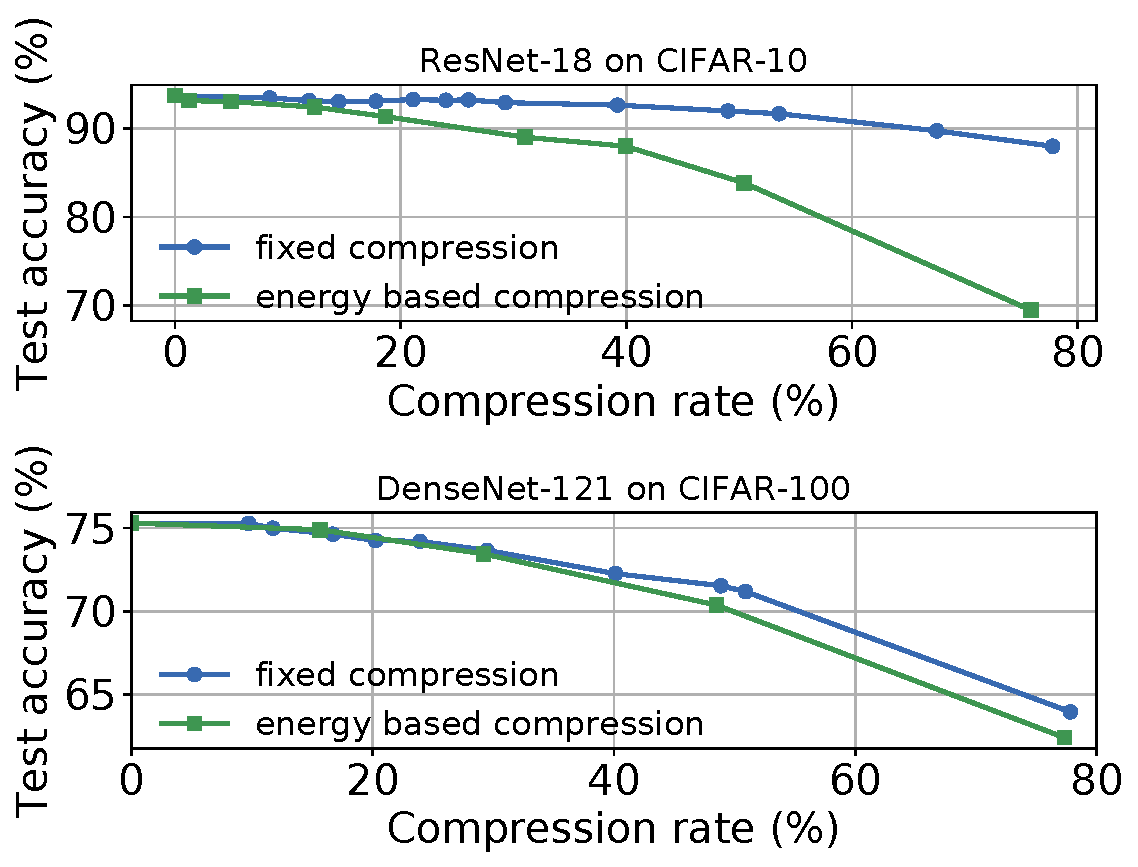
\includegraphics[width=1.0\columnwidth]{cifars-accuracy-compress-font6.pdf}
  \caption{{\it Test accuracy as a function of the compression rate for ResNet-18 on CIFAR-10 and DenseNet-121 on CIFAR-100. The fixed compression scheme that uses the same compression rate for each layer gives the highest test accuracy.}}
  \label{fig:energy-static-compression-compare}
\end{figure}


First, we study how band-limiting training effects the final test accuracy of two popular deep neural networks, namely, ResNet-18 and DenseNet-121, on CIFAR-10 and CIFAR-100 datasets, respectively. Specifically, we vary the compression rate between 0\% and 50\% for each convolutional layer (i.e., the percentage of coefficients discarded) and we train the two models for 350 epochs. Then, we  measure the final test accuracy using the same compression rate as the one used during training. Our results in Table~\ref{tab:final-accuracies} show a smooth degradation in accuracy despite the aggressive compression applied during band-limiting training.

To better understand the effects of band-limiting training, in Figure~\ref{fig:energy-static-compression-compare}, we explore two different compression schemes: (1) fixed compression, which discards the same percentage of spectral coefficients in each layer and (2) energy compression, which discards coefficients in an adaptive manner based on the specified energy retention in the frequency spectrum. %The energy $E(x)$ of an input tensor $x$ is defined as sum of energies (squares of the amplitudes $|x[i]|$) at every position. 
By Parseval's theorem, the energy of an input tensor $x$ is preserved in the Fourier domain and defined as: $E(x) = \sum_{n=0}^{N-1} |x[n]|^2 = \sum_{\omega=0}^{2\pi} |F_x[\omega]|$ (for normalized FFT transformation). 
For example, for two convolutional layers of the same size, a fixed compression of 50\% discards 50\% of coefficients in each layer. On the other hand, the energy approach may find that 90\% of the energy is preserved in the 40\% of the low frequency coefficients in the first convolutional layer while for the second convolutional layer, 90\% of energy is preserved in 60\% of the low frequency coefficients. %Thus, the overall compression amounts to the same value of 50\% in both static and energy based compression methods. We apply the same scheme to every convolutional layer.

For more than 50\% of compression rate for both techniques, %(the precise compression ratios are 53.53\% and 53.74\%, respectively), 
the fixed compression method achieves the max test accuracy of 92.32\% (only about 1\% worse than the best test accuracy for the full model) whereas the preserved energy method results in significant losses (e.g., ResNet-18 reaches 83.37\% on CIFAR-10). Our findings suggest that altering the compression rate during model training may affect the dynamics of SGD. The worse accuracy of the models trained with any form of dynamic compression is result of the higher noise incurred by frequent changes to the number of coefficients that are considered during training. The test accuracy for energy-based compression follows the coefficient one for DenseNet-121 while they markedly diverge for ResNet-18. ResNet combines outputs from $L$ and $L+1$ layers by summation. In the adaptive scheme, this means adding maps produced from different spectral bands. In contrast, DenseNet concatenates the layers.

% FIGURE
\begin{figure}[t]
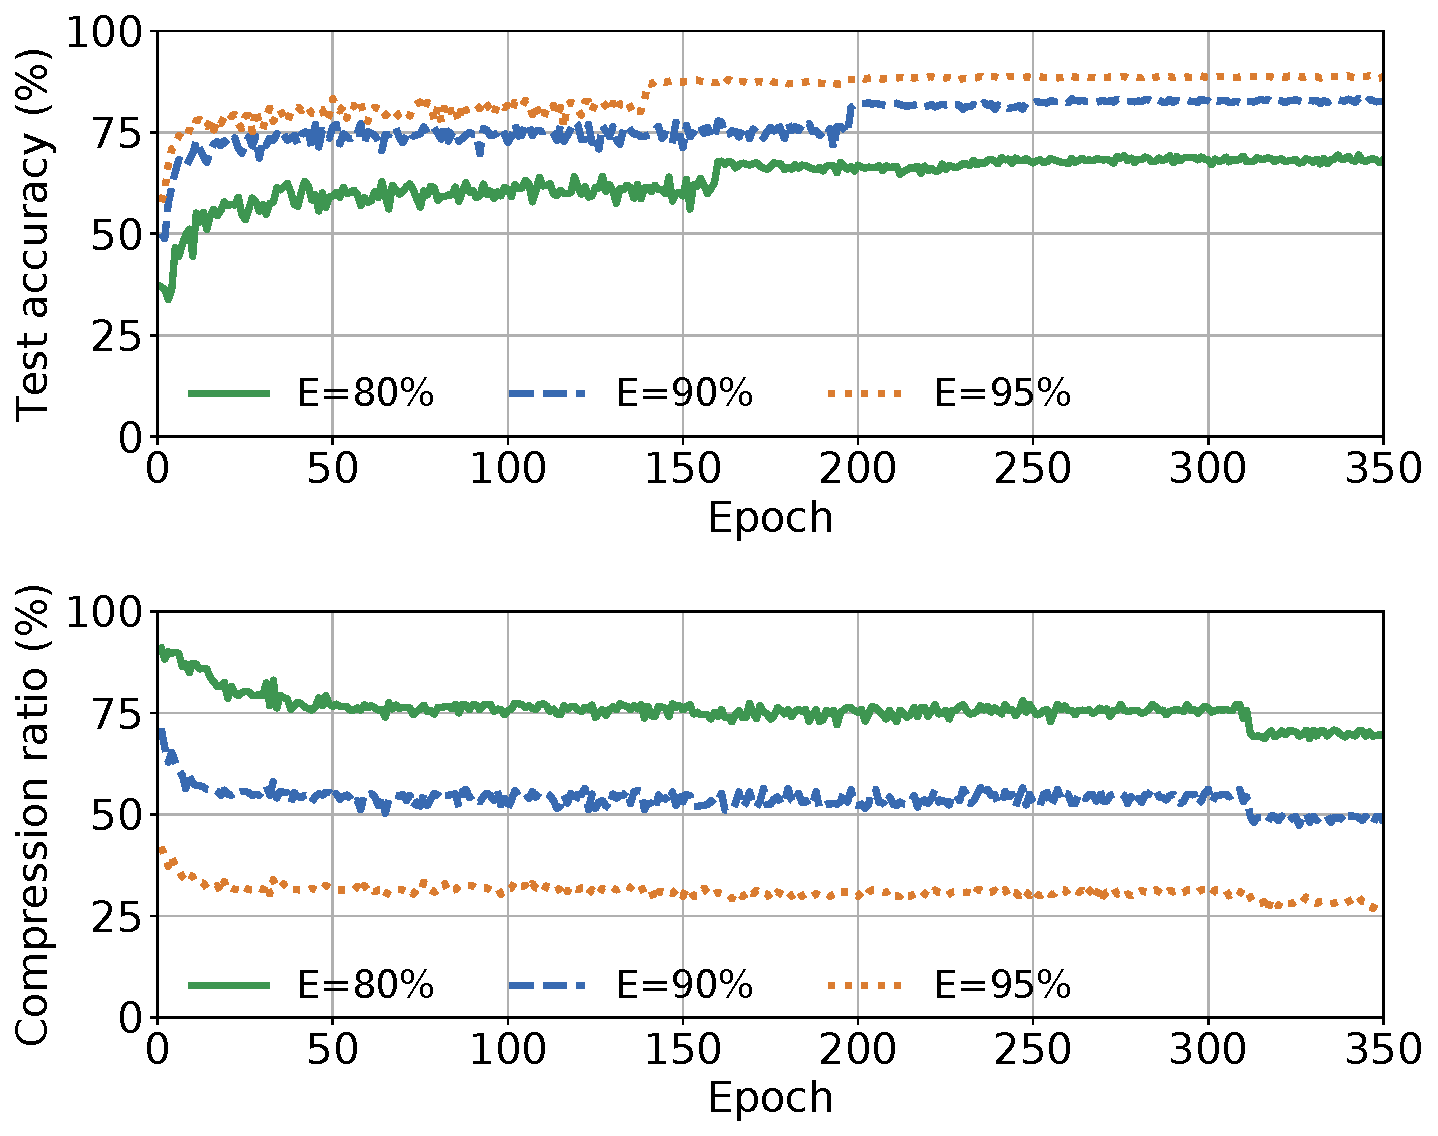
\includegraphics[scale=0.33]{bandwidth-changes-font2.pdf}
  \caption{{\it Compression changes during training with constant energy preserved: the longer we train the models with the same energy preserved, the smaller compression is applied. The compression rate (\%) is calculated based on the size of the intermediate results for the FFT based convolution. E - is the amount of energy (in \%) preserved in the spectral representation: 80, 90 and 95. We trained ResNet-18 models on CIFAR-10 for 350 epochs. The best test accuracy levels achieved by the models are: 69.47\%, 83.37\% and 88.99\%, respectively.}}
  \label{fig:dynamicCompressionChanges}
\end{figure}

% \vspace{1em}
To dive deeper into the effects on SGD, we performed an experiment where we keep the same energy preserved in each layer and for every epoch. Every epoch we record what is the physical compression (number of discarded coefficients) for each layer. The dynamic compression based on the energy preserved shows that at the beginning of the training the network is focused on the low frequency coefficients and as the training unfolds, more and more coefficients are taken into account, which is shown in Figure~\ref{fig:dynamicCompressionChanges}. The compression based on preserved energy does not steadily converge to a certain compression rate but can decrease significantly and abruptly even at the end of the training process (especially, for the initial layers).

% \iffalse
% \subsection{Per-Operation Error}
% Despite the accurate predictive performance of the trained models, we find that the approximation error in the individual convolution operations to be relatively high.
%  We executed our convolution operation with compression for different compression rates on a single CIFAR-10 image. The compression was measured relatively to the execution of our bandlimited convolution without any compression (100\% of the energy of the input image is preserved). The results show that the relative error is already high (about 22.07\%) for a single index discarded (the smallest possible compression of about 6\%) in Figure~\ref{fig:compareErrorsFFT2Dconv}. 
 
%  This result is a mathematically curious point. Why are models trained with bandlimited convolutions so accurate when the individual convolution operations are not? All of our experimental results suggest that bandlimiting is not simply an operator-level approximation, but rather, the \emph{network learns to use the low-frequency coefficients to make predictions.} 

% \begin{figure}[t]
%   \centering
%   
\includegraphics[width=\linewidth]{figures/RelativeErrorConv2D/conv2DrelativeErrorGraph3.pdf} %width=\linewidth]
%   \caption{{\it A comparison of the relative (in \%) and absolute errors between 2D convolution from PyTorch (which is our gold standard with high numeric accuracy) and a fine-grained top compression method for a CIFAR-10 image and a 5x5 filter (with 3 channels).
% }}
%   \label{fig:compareErrorsFFT2Dconv}
% \end{figure}
% \fi

% FIGURE
\begin{figure}[t]
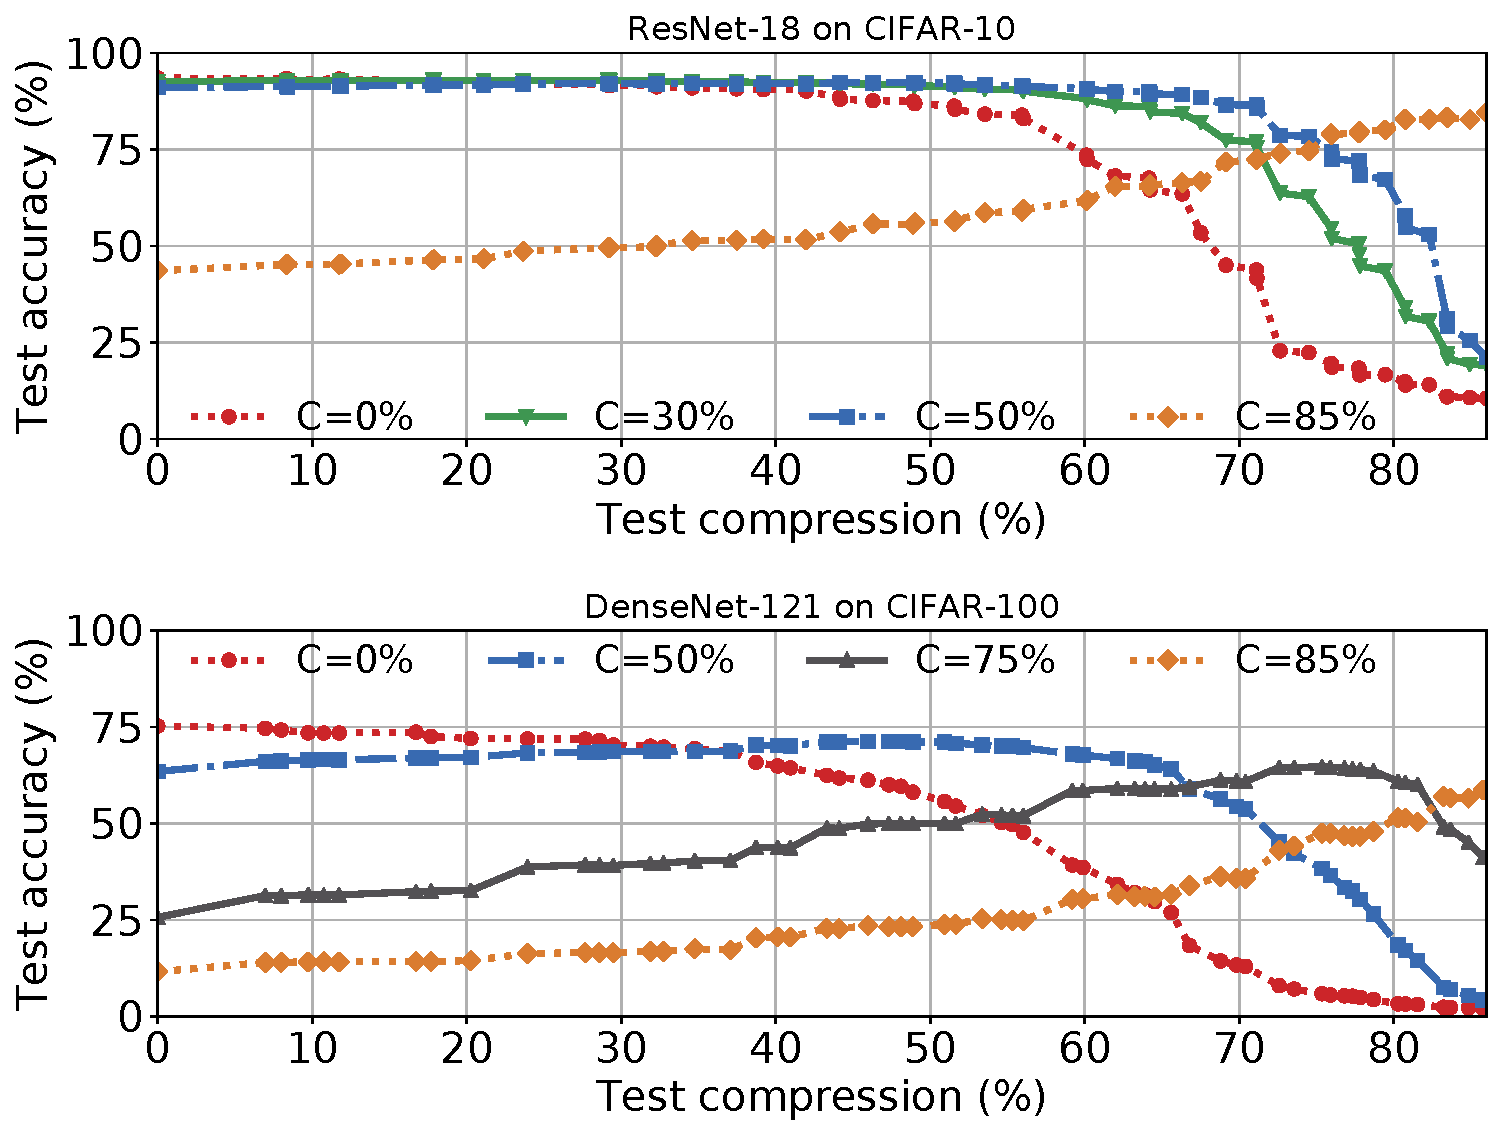
\includegraphics[scale=0.33]{test-train-font2.pdf}
  \caption{{\it The highest accuracy during testing is for the same compression level as used for training and the test accuracy degrades smoothly for higher or lower levels of compression.
  First, we train models with different compression levels (e.g. DenseNet-121 on CIFAR-100 with compression rates: 0\%, 50\%, 75\%, and 85\%). Second, we test each model with compression levels ranging from 0\% to 85\%.}}
  \label{fig:compressionLevelsTrainTest2D}
\end{figure}

\subsection{Training Compression vs. Inference Compression} 
Having shown a smooth degradation in performance for various compression rates, we now study the effect of changing the compression rates during training and inference phases. This scenario is useful during dynamic resource allocation in model serving systems.

Figure~\ref{fig:compressionLevelsTrainTest2D} illustrates the test accuracy of ResNet-18 and DenseNet-121 models trained with specific coefficient compression rates (e.g., 0\%, 50\%, and 85\%) while the compression rates are changed systematically during inference. We observe that the models achieve their best test accuracy when the same level of compression is used during training and inference. In addition, we performed the same experiment across 25 randomly chosen time-series datasets from the UCR archive~\cite{UCRArchive} using a 3-layer Fully Convolutional Network (FCN), which has achieved state-of-the-art results in prior work~\cite{FCN2017}. We used the Friedman statistical test~\cite{friedman1937use} followed by the post-hoc Nemenyi test~\cite{nemenyi1962distribution} to assess the performance of multiple compression rates during inference over multiple datasets (see supplementary material for details). Our results suggest that the best test accuracy is achieved when the same compression rate is used during training and inference and, importantly, the difference in accuracy is statistically significantly better in comparison to the test accuracy achieved with different compression rate during inference.

Overall, our experiments show that band-limited CNNs learn the constrained spectrum and perform the best for similar constraining during inference. In addition, the smooth degradation in performance is a valuable property of band-limited training as it permits outer optimizations to tune the compression rate parameter without unexpected instabilities or performance cliffs.

\begin{table}[t]
\caption{Resource utilization (RES. in \%) for a given precision and compression rate (SETUP). MEM. ALLOC. - the memory size allocated on the GPU device, MEM. UTIL. - percent of time when memory was read or written, GPU UTIL. - percent of time when one or more kernels was executing on the GPU. C - denotes the compression rate (\%) applied, e.g., FP32-C=50\% is model trained with 32 bit precision for floating point numbers and 50\% compression applied.}
\label{tab:micro-analysis}
\vskip 0.15in
\begin{center}
\begin{small}
\begin{sc}
\begin{tabular}{lrrrr}
\toprule
\multicolumn{1}{p{0.8cm}}{\centering \backslashbox{res(\%)}{setup}} & \multicolumn{1}{p{0.8cm}}{\centering fp32-C=0\%} & \multicolumn{1}{p{0.8cm}}{\centering fp16-C=0\%} & \multicolumn{1}{p{0.8cm}}{\centering fp32-C=50\%} & \multicolumn{1}{p{0.8cm}}{\centering fp32-C=85\%} \\
\midrule
Avg. Mem. alloc. & 6.69 & 4.79 & 6.45 & 4.92 \\
Max. Mem. alloc. & 16.36 & 11.69 & 14.98 & 10.75 \\
Avg. Mem. util. & 9.97 & 5.46 & 5.54 & 3.50 \\
Max. Mem. util. & 41 & 22 & 24 & 20 \\
Avg. GPU util. & 24.38 & 22.53 & 21.70 & 16.87 \\
Max. GPU util. & 89 & 81 & 74 & 70 \\
\midrule
Test Acc. & 93.69 & 91.53 & 92.32 & 85.4 \\
\bottomrule
\end{tabular}
\end{sc}
\end{small}
\end{center}
\vskip -0.1in
\end{table}

\subsection{Comparison Against Reduced Precision Method}
Until now, we have demonstrated the performance of band-limited CNNs in comparison to the full spectra counterparts. It remains to show how the compression mechanism compares against a strong baseline. Specifically, we evaluate band-limited CNNs against CNNs using reduced precision arithmetic (RPA). RPA-based methods require specialized libraries~\footnote{https://devblogs.nvidia.com/apex-pytorch-easy-mixed-precision-training/} and are notoriously unstable. They require significant architectural modifications for precision levels under 16-bits--if not new training chipsets~\cite{wang2018training, abergerhigh}.
 %~\footnote{PyTorch delegates the selection of the convolution algorithm to NVIDIA's cuDNN.} 
%\textbf{**What algorithm is AMP using for convolution? Is this even apples-to-apples?**}
From a resource perspective, band-limited CNNs are competitive with RPA-based CNNs--without requiring specialized libraries. To record the memory allocation, we run ResNet-18 on CIFAR-10 with batch size 32 and we query the VBIOS (via nvidia-smi
%~\footnote{https://bit.ly/2SZryG8})
every millisecond in the window of 7 seconds). Table~\ref{tab:micro-analysis} shows a set of basic statistics for resource utilization for RPA-based (fp16) and band-limited models. The more compression is applied or the lower the precision set (fp16), the lower the utilization of resources. %Interestingly, there is actually a significant saving in terms of computation in comparison to the RPA-based method. 
In the supplementary material we show that it is possible to combine the two methods.

\subsection{Robustness to Noise}
%\textbf{**? Take the trained FP16 model and FP32-50 model perturb input images by Gaussian Noise, plot loss in accuracy?**}

% FIGURE
Next, we evaluate the robustness of band-limited CNNs. Specifically, models trained with more compression discard part of the noise by removing the high frequency Fourier coefficients. In Figure~\ref{fig:gaussian-noise}, we show the test accuracy for input images perturbed with different levels of Gaussian noise, which is controlled systematically by the sigma parameter, fed into models trained with different compression levels (i.e., 0\%, 50\%, and 85\%) and methods (i.e., band-limited vs. RPA-based). Our results demonstrate that models trained with higher compression are more robust to the inserted noise. Interestingly, band-limited CNNs also outperform the RPA-based method and under-fitted models (e.g., via early stopping), which do not exhibit the robustness to noise.

We additionally run experiments using Foolbox~\cite{foolbox}. Our method is robust to decision-based and score-based (black-box) attacks (e.g., the band-limited model is better than the full-spectra model in 70\% of cases for the additive uniform noise, and in about 99\% cases for the pixel perturbations attacks) but not to the gradient-based (white-box and adaptive) attacks, e.g., Carlini-Wagner~\cite{Carlini2017Towars} (band-limited convolutions return proper gradients). Fourier properties suggest further investigation of invariances under adversarial rotations and translations~\cite{madry2017rotation}.

\begin{figure}[t]
\centering
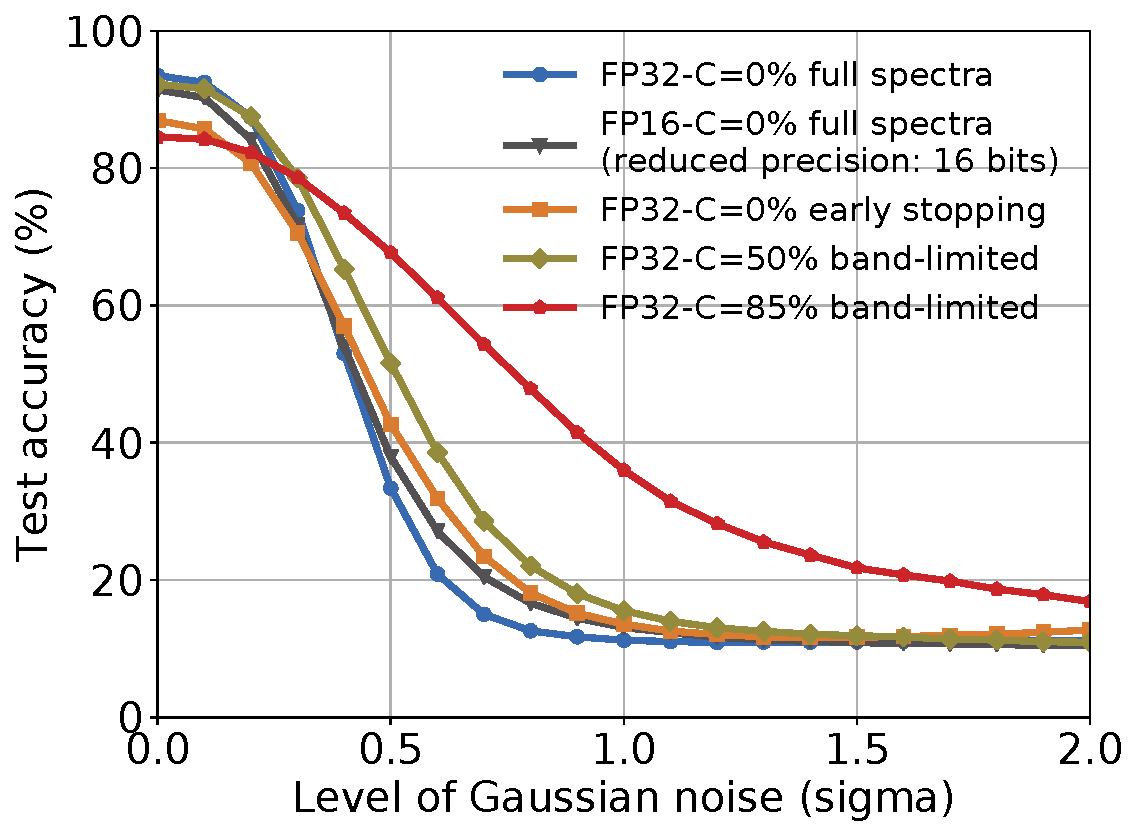
\includegraphics[width=0.8\columnwidth]{gaussian_noise_font.pdf}
\caption{{\it Input test images are perturbed with Gaussian noise, where the sigma parameter is changed from 0 to 2. The more band-limited model, the more robust it is to the introduced noise. We use ResNet-18 models trained on CIFAR-10.}}
  \label{fig:gaussian-noise}
\end{figure}

\subsection{Control of the GPU and Memory Usage}

\begin{figure}[t]
\centering
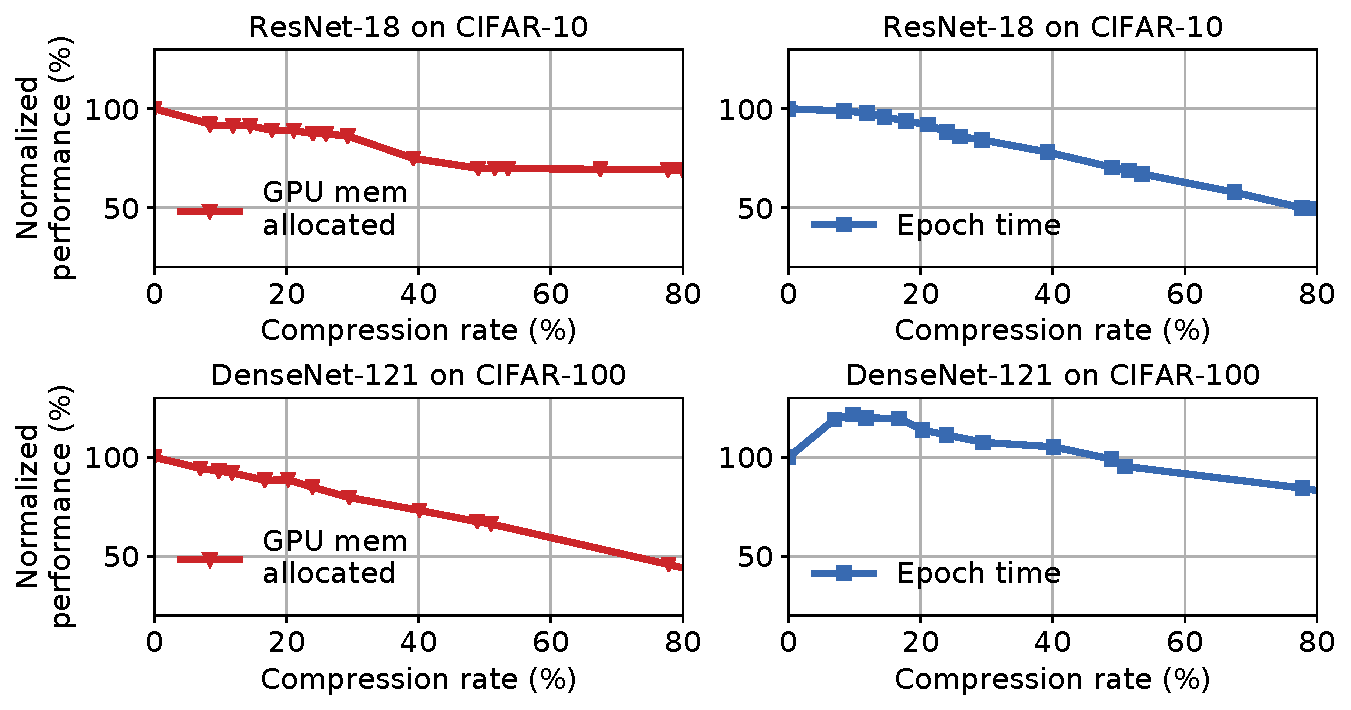
\includegraphics[width=0.8\columnwidth]{gpu_time_mem_alloc_font3.pdf}
%width=\linewidth]
\caption{{\it Normalized performance (\%) between models trained with different FFT-compression rates.}}
\label{fig:normalized_performance}
\end{figure}

In Figure~\ref{fig:normalized_performance}, we compare two metrics: maximum GPU memory allocated (during training) and time per epoch, as we increase the compression rate. The points in the graph with 100\% performance for 0\% of compression rate correspond to the values of the metrics for the full spectra (uncompressed) model. We normalize the values for the compressed models as: $\frac{\text{metric value for a compressed model}}{\text{metric value for the full spectra model}} \cdot 100\%$. 

For the ResNet-18 architecture, a small drop in accuracy can save a significant amount of computation time. However, for more convolutional layers in DenseNet-121, the overhead of compression (for small compression rate) is no longer amortized by fewer multiplications (between compressed tensors). The overhead is due to the modifications of tensors to compress them in the frequency domain and their decompression (restoration to the initial size) before going back to the spatial domain (to preserve the same frequencies for the inverse FFT). FFT-ed tensors in PyTorch place the lowest frequency coefficients in the corners. For compression, we extract parts of a tensor from its top-left and bottom-left corners. For the decompression part, we pad the discarded parts with zeros and concatenate the top and bottom slices. %These operations have a non-negligible cost. The overhead might be minimized in 2D case if the DC component would be moved to the center and the compression would only extract the middle coefficients (by slicing and without a need to stitch together different parts of a tensor) so that the compressed tensor would remain contiguous.

DenseNet-121 shows a significant drop in GPU memory usage with relatively low decrease in accuracy. On the other hand, ResNet-18 is a smaller network and after about 50\% of the compression rate, other than convolutional layers start dominate the memory usage. The convolution operation remains the major computation bottleneck and we decrease it with higher compression. %For ResNet-50 on ImageNet, we observe a substantial drop in memory usage after applying our compression and similar behavior in terms of the time per epoch to the ResNet-18 model on CIFAR-10.

\subsection{Generality of the Results} To show the applicability of band-limited training to different domains, we apply our technique using the FCN architecture discussed previously on the time-series datasets from the UCR archive. Figure~\ref{fig:AccuracyCompareConv1DFCN-UCR} compares the test accuracy between full-spectra (no compression) and band-limited (with 50\% compression) models with FFT-based 1D convolutions. % on time-series datasets from the UCR archive. 
As with the results for 2D convolutions, we find that not only is accuracy preserved but there are very significant savings in terms of GPU memory usage (Table~\ref{tab:accuracy-mem-usage-conv1}).

%FIGURE
\begin{figure}[t]
\centering
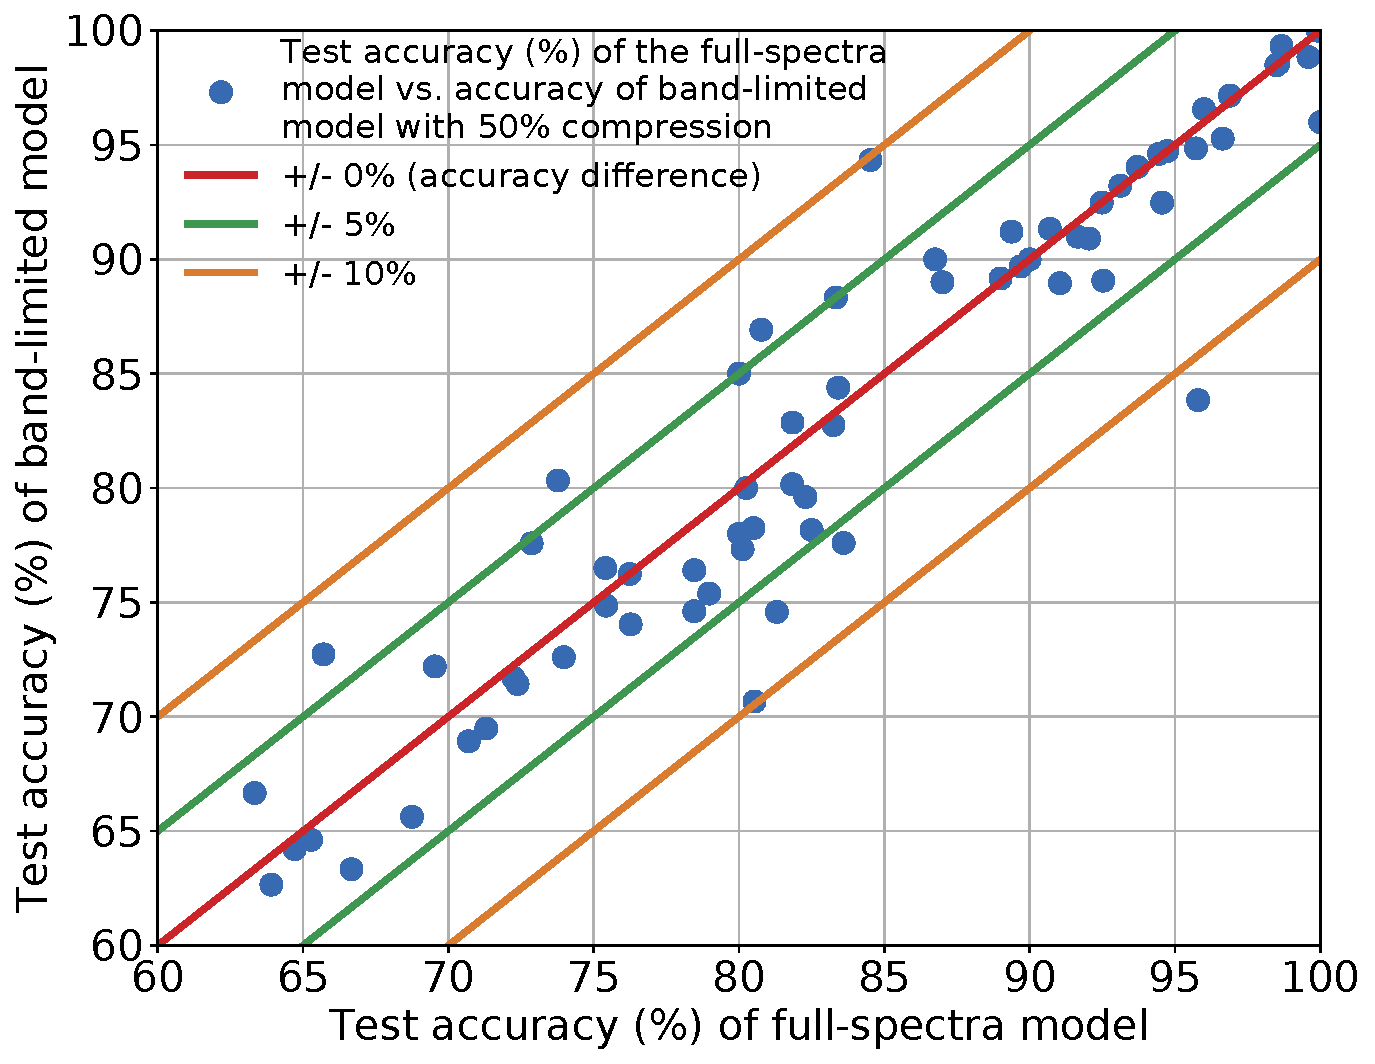
\includegraphics[scale=0.28]{time-series-font2.pdf}
  \caption{{\it Comparing test accuracy (\%) on a 3-layer FCN architecture between full-spectra models (100\% energy preserved, no compression) and a band-limited models with 50\% compression rate for time-series datasets from the UCR archive. The red line indicates no difference in accuracy between the models while green and orange margin lines show +/- 5\% and +/- 10\% differences.}}
  \label{fig:AccuracyCompareConv1DFCN-UCR}
\end{figure}

\begin{table}[ht!]
\caption{Resource utilization and accuracy for the FCN network on a representative time-series dataset (see supplement for details).}
\label{tab:accuracy-mem-usage-conv1}
\begin{center}
\begin{small}
\begin{sc}
\begin{tabular}{ccc}
\toprule
\multicolumn{1}{p{2.3cm}}{\centering Energy\\preserved (\%)} & \multicolumn{1}{p{2.3cm}}{\centering Avg. GPU mem\\usage (MB)} & \multicolumn{1}{p{2.3cm}}{\centering Max. test\\ accuracy (\%)} \\
\midrule
100 & 118 & 64.40 \\
%99 & 41 & 61.98 \\
%98 & 34 & 60.66 \\
\textbf{90} & \textbf{25} & \textbf{63.52} \\
50 & 21 & 59.34 \\
10 & 17 & 40.00 \\
\bottomrule
\end{tabular}
\end{sc}
\end{small}
\end{center}
\end{table}

%\subsection{Additional experimental results}



